\documentclass[11pt,a4paper]{article}
\usepackage[latin1]{inputenc}
\usepackage{amsmath}
\usepackage{microtype}
\usepackage[none]{hyphenat}
\usepackage{verbatim}
\usepackage{amsfonts}
\usepackage{amssymb}
\usepackage{enumitem}
\renewcommand{\familydefault}{\sfdefault}
\usepackage{mathpazo}
\renewcommand{\rmdefault}{put}
\usepackage{enumitem}
\usepackage[dvipsnames,svgnames]{xcolor}
\usepackage{tkz-euclide}
\usetkzobj{all}
\usepackage{graphicx}
\usepackage{tikz} 	
\usepackage{adjustbox}
\usepackage{multicol}
\usepackage{lipsum}
\usepackage[left=0.7cm,right=1cm,top=1cm,bottom=1.5cm]{geometry}
\usepackage{cancel} \usepackage{xcolor}
\usepackage{tcolorbox}
\usetikzlibrary{decorations.pathmorphing,patterns}
\usetikzlibrary{decorations.pathreplacing,calc}
 \newcommand\coret[2][red]{\renewcommand\CancelColor{\color{#1}}\cancel{#2}}
\SetLabelAlign{Center}{\hfil\makebox[1.0em]{#1}\hfil}

%%_------= solusi


% Set this =0 to hide, =1 to show

% Set this =0 to hide, =1 to show
\newtcolorbox{mybox}[1][] { colframe = blue!10, colback = blue!3,boxsep=0pt,left=0.2em, coltitle = blue!20!black, title = \textbf{jawab}, #1, } 

%---------- kunci (jika 1 ) muncul
\def\tampilkunci{1}
\newcommand{\hide}[1]{\ifnum\tampilkunci=1
%
\begin{mybox}
 #1
\end{mybox}
%
\vspace{\baselineskip}\fi\ifnum\tampilkunci=0
%
\vspace{1cm}
%
\fi}



\newcommand*\cicled[1]{\tikz[baseline=(char.base)]{\node[white, shape=circle, fill=red!80,draw,inner sep=0.5pt](char){#1};}}

\newcommand*\kunci[1]{\ifnum\tampilkunci=1
%
\tikz[baseline=(char.base)]{\node[red, shape=circle,draw,inner sep=0.5pt,xshift=2pt](char){#1};}\stepcounter{enumii}
\fi\ifnum\tampilkunci=0
%
\hspace{3pt}#1\stepcounter{enumii}
%
\fi}

\newcommand*\silang[1]{\tikz[baseline=(char.base)]{
\draw[red,thick](-0.2,-0.20)--(0.2,0.2);
\draw[red,thick](-0.2,0.20)--(0.2,-0.2);
\node[black](char){#1};
}}

\newcommand*\centang[1]{\tikz[baseline=(char.base)]{
\draw[red, very thick](-0.2,0.1)--(-0.1,0)--(0.2,0.3);
\node(char){#1};
}}

\newcommand*\merah[1]{
\textcolor{red}{#1}}
\newcommand*\pilgan[1]{
\begin{enumerate}[label=\Alph*., itemsep=0pt,topsep=0pt,leftmargin=*,align=Center] #1 
\end{enumerate}}
\newcommand*\pernyataan[1]{
\begin{enumerate}[label=(\arabic*), itemsep=0pt,topsep=0pt,leftmargin=*] #1 
\end{enumerate}}

\newcommand{\pilgani}[1]{                            \vspace{-0.3cm}\begin{multicols}{2}
 \begin{enumerate}[label=\Alph*., itemsep=0pt,topsep=0pt,leftmargin=*,align=Center]#1                     \end{enumerate}
 \phantom{ini cuma sapi, wedus, dan ayam}
 \end{multicols}}
\newcommand{\spasi}{
    \vspace{-0.5cm}
\begin{tcolorbox} [boxrule=0.5pt,height=4.2cm, colback=white]

\end{tcolorbox}

}


\begin{document}

\begin{multicols*}{2}
\begin{enumerate}
% no1---------------
\item Hasil pengukuran yang benar adalah menjumlahkan masing-masing lengan, yakni 150 + 20 + 3 = 173 gram. Jawabannya \textbf{D}

% no2 ------------------
\item Rute petugas pos digambar sehingga bisa menunjukkan perpindahan dari posisi awal dan akhir

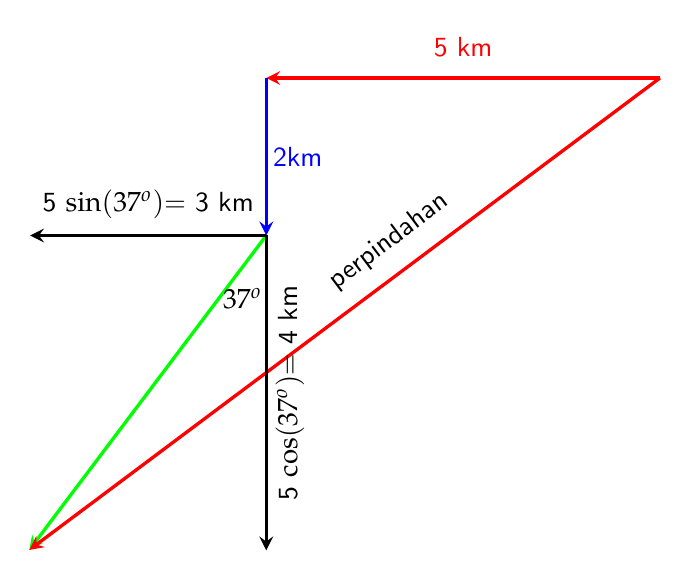
\begin{tikzpicture}
\draw[very thick, red,-stealth](0,0) -- node [midway,yshift=0.4cm]{5 km}(-5,0) ;
\draw[very thick, blue,-stealth](-5,0) -- node [midway,xshift=0.4cm]{2km}(-5,-2);
\draw[very thick, green, -stealth](-5,-2)--+ (233:5) coordinate (A);
\draw[very thick, red,- stealth](0,0) -- node [midway, rotate=37, black,yshift=0.4cm,xshift=1cm]{perpindahan}(A);
\draw[very thick, black,- stealth](-5,-2) -- node [midway, yshift=0.4cm]{5 $\sin(37^o)$= 3 km} (-8,-2);
\node at (-5.3,-2.8) {$37^o$};
\draw[very thick, black,- stealth](-5,-2) -- node [midway, xshift=0.3cm, rotate = 90]{5 $\cos(37^o)$= 4 km} (-5,-6);
\end{tikzpicture}

\begin{tabular}{p{1cm}  p{2cm} p{2cm}}
&$r_x$ & $ r_y$\\ 
1 & -5 km & 0 \\
2 & 0 & -2 km \\
3 & - 3 km & -4 km\\\hline
$\Sigma$ & -8 km & - 6 km 
\end{tabular}

Sehingga resultan perpindahannya adalah $r =\sqrt{(-8)^2 + (-6)^2} = 10$ km. \textbf{A}



% no3 ----------------------------
\item Jarak yang ditempuh benda selama 12 detik sama dengan jumlah luasan di bawah grafik (di atas garis sumbu $t$ dan di bawahnya)





\end{enumerate}


\end{multicols*}
\end{document}






